\vspace{-2mm}
\section*{Problem 1}
\vspace{-2mm}
    \subsection*{code 1}
        \begin{listing}[h!]
        \inputminted[framerule = 1pt,framesep = 2mm , frame = lines, fontsize=\footnotesize]{python}{./code/report_03/01.py}
        \vspace{-3mm}
        \caption{01.py}
        \end{listing}
    \vspace{-5mm}
    
    \subsection*{problem 1 description}
    기본적인 instance 생성시 constructor method의 추가와 클래스 내부의 \mintinline{python}{__str__} method를 통해서 print 함수의 인자로 출력될때 문제와 같은 출력이 될 수 있도록 작성해 주었다.
    간단한 클래스간의 상속을 통해서 속성값이 전달되는 부분도 확인할 수 있었다.
\vspace{-2mm}
\section*{Problem 2}
\vspace{-2mm}
    \subsection*{code 2}
        \begin{listing}[h!]
        \inputminted[framerule = 1pt,framesep = 2mm , frame = lines, fontsize=\footnotesize]{python}{./code/report_03/02.py}
        \vspace{-3mm}
        \caption{02.py}
        \end{listing}
    \vspace{-5mm}
\clearpage
    \subsection*{problem 2 description}
    \mintinline{python}{__eq__} method를 설정해주어서 클래스 내부 변수간의 동일한 point 인지를 판단하는 \mintinline{python}{=} 연산에 대해서 x 와 y point value가 모두 동일한 부분을 설정
\vspace{-2mm}
\section*{Problem 3}
\vspace{-2mm}
    \subsection*{code 3}
        \begin{listing}[h!]
        \inputminted[framerule = 1pt,framesep = 2mm , frame = lines, fontsize=\footnotesize]{python}{./code/report_03/03.py}
        \vspace{-3mm}
        \caption{03.py}
        \end{listing}
    \vspace{-5mm}
    
    \subsection*{problem 3 description}
    부모 class와 상속을 받는 클래스간의 공통 속성에 대해서 \mintinline{python}{super().__init__()} 을 이용해 constructor를 설정
\section*{Problem 4}
\vspace{-2mm}    
    \subsection*{problem 4 description}
    문제에 주어진 \mintinline{python}{__str__()} 와 \mintinline{python}{__add__()} method 의 경우 \mintinline{python}{main.py}에서 각각 print 에서 instance를 str로 출력하는 구문과 문제의 설명부분에서 기술된 \mintinline{python}{Student.get_id()} 에서 형변환에 따른 클래스 멤버 변수간의 \mintinline{python}{+} 연산이 클래스에서 선언된 다른 instance간의 구문이 없기 때문에 각각 \mintinline{python}{pass} 해주었다.
    
    \mintinline{python}{Student.get_id()} 에서 문제의 조건대로 str type으로 name의 첫 글자들의 아스키 코드를 
    연결해준 값과 각 \mintinline{python}{first_name}, \mintinline{python}{last_name}의 string을 list로 형변환해주어 iterable하게 만든후 이를 아스키코드로 변환해주는 \mintinline{python}{ord()} 와 \mintinline{python}{map()} 을 이용해 list로 저장후 \mintinline{python}{sum} 을 이용해 각각의 합을 모두 구해준 후 앞서 구한 결과와 더해주어 
    student \#을 구하였다.
\clearpage
    \subsection*{code 4}
        \begin{listing}[h!]
        \inputminted[framerule = 1pt,framesep = 2mm , frame = lines, fontsize=\footnotesize]{python}{./code/report_03/04.py}
        \vspace{-3mm}
        \caption{04.py}
        \end{listing}
    \vspace{-5mm}
\clearpage
\section*{Appendix : code print out}
\vspace{-2mm}
    \begin{figure}[!h]\centering
		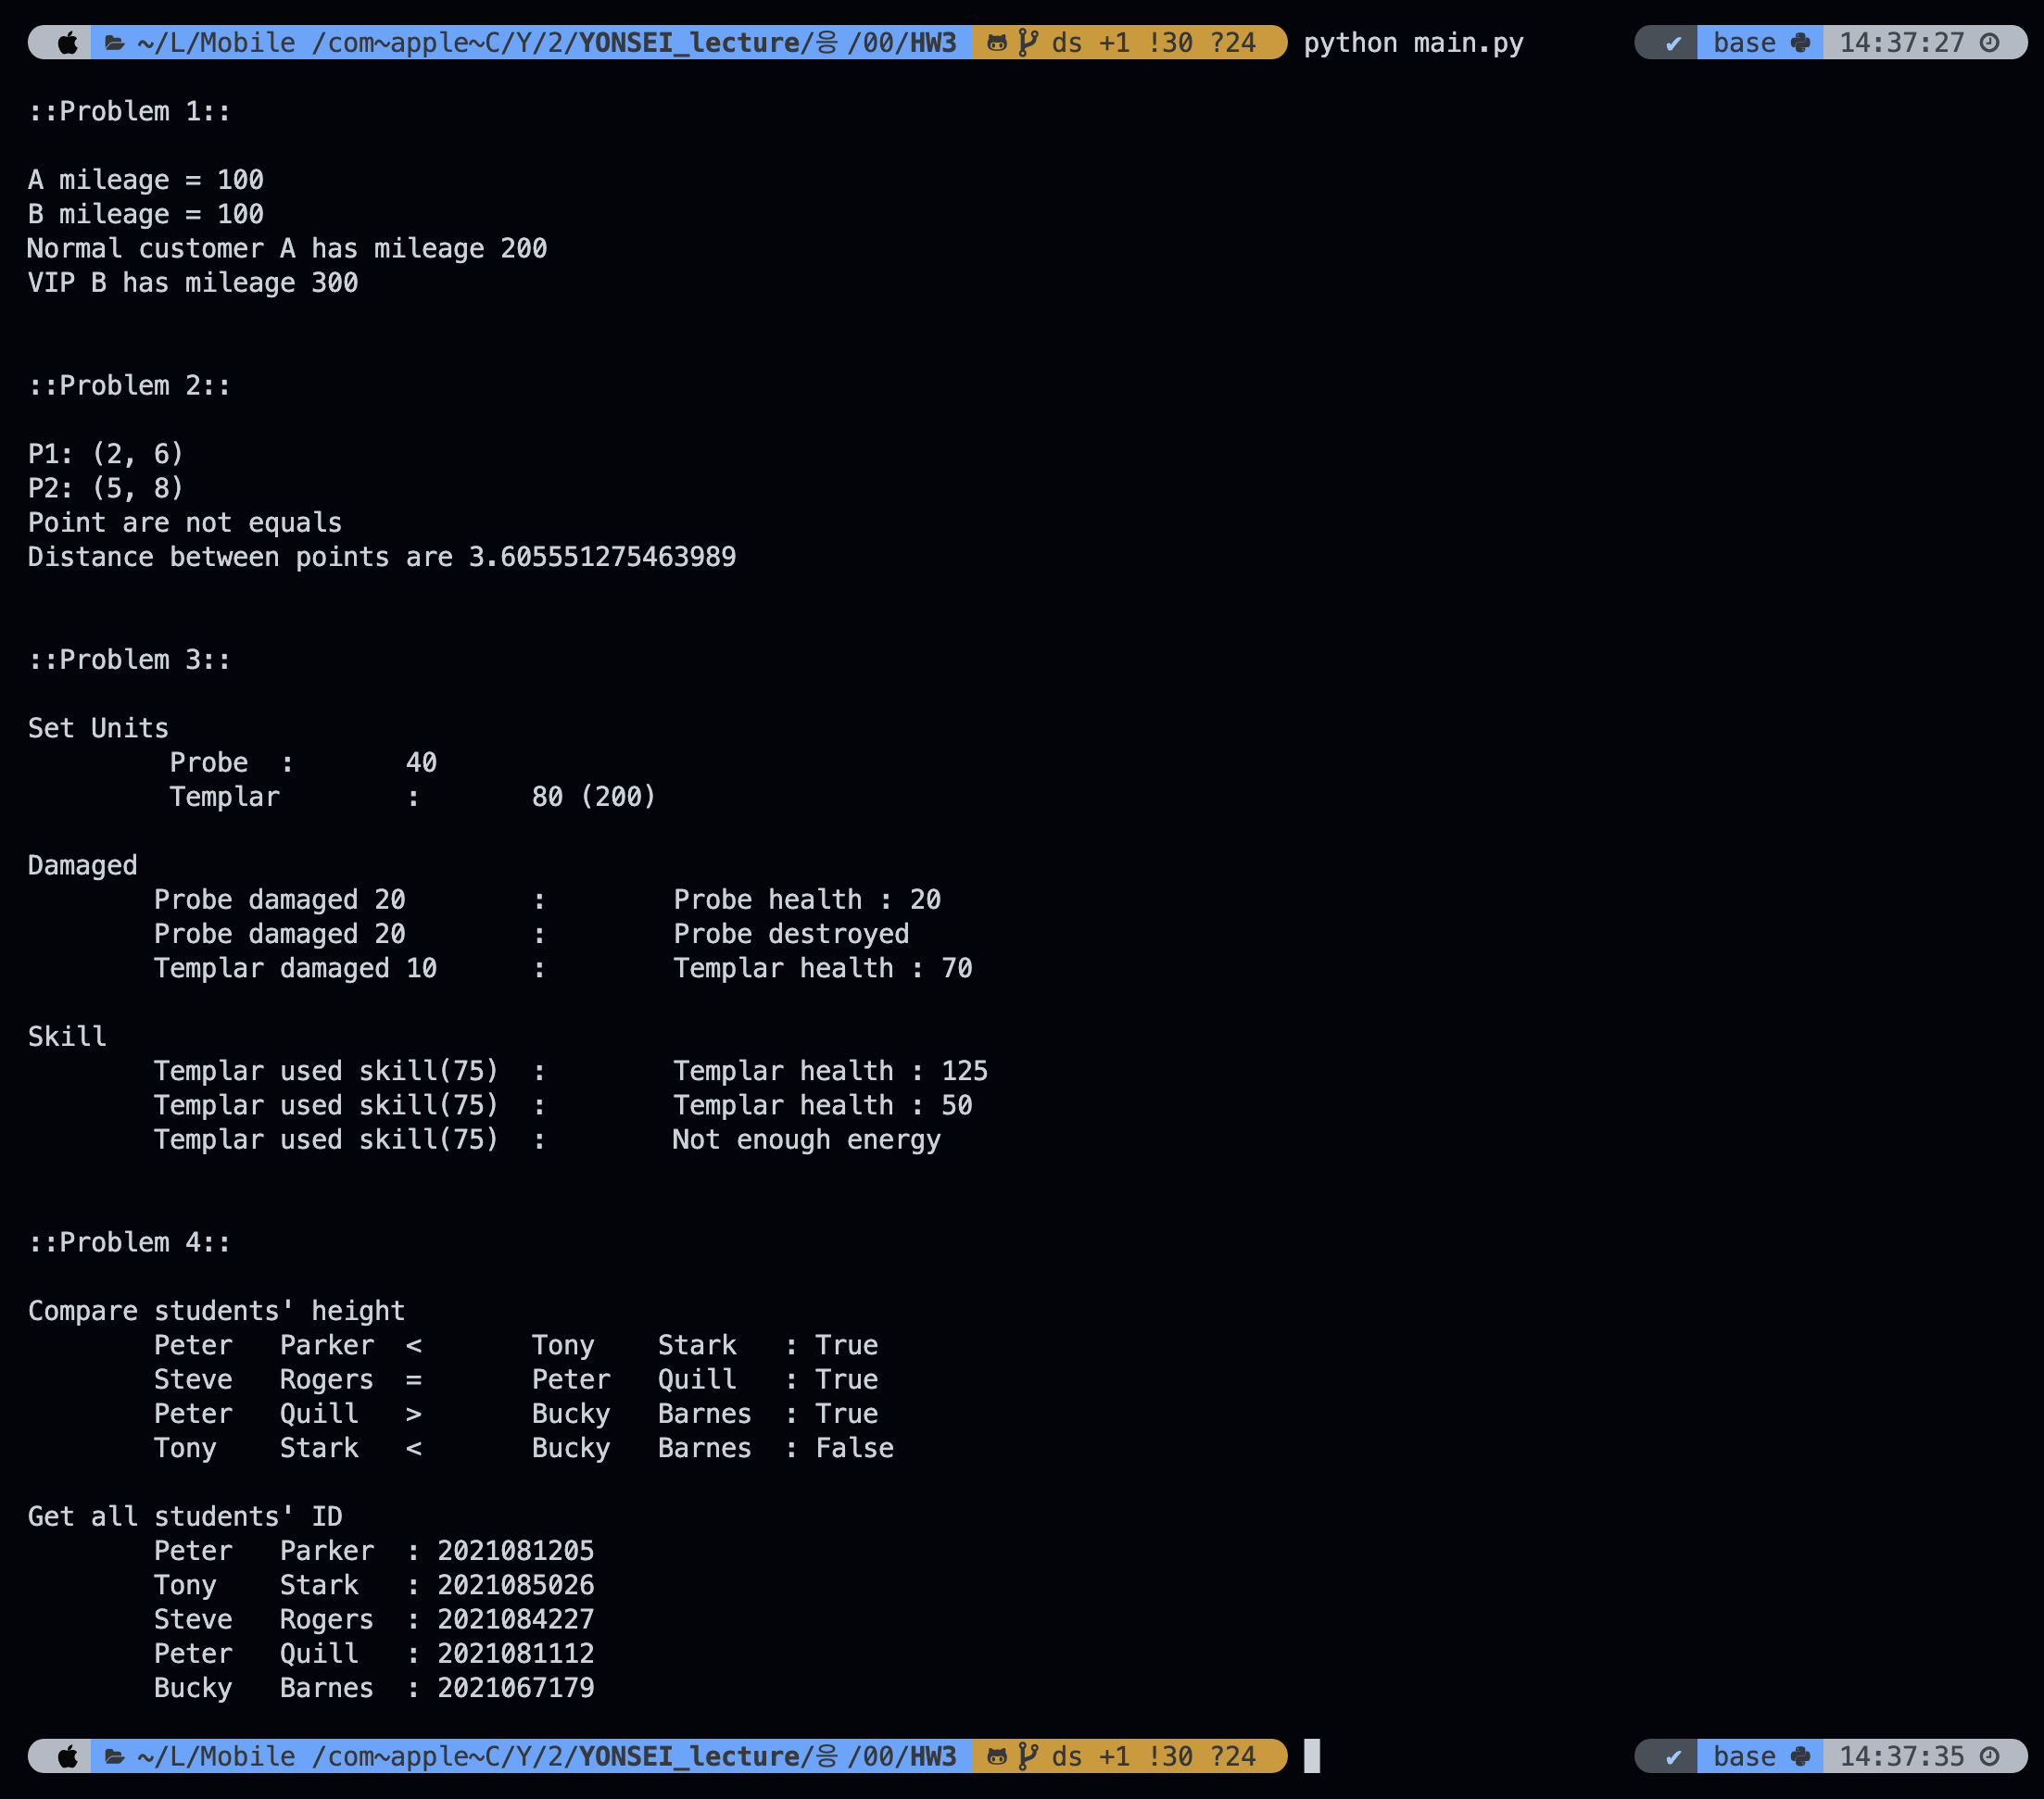
\includegraphics[width=\textwidth]{image/report_03/01.png}
		\caption{\small \mintinline{python}{main.py} Print Out}
		\vspace{-10pt}
    \end{figure}